\documentclass[14pt]{article}
\usepackage{sbc-template}
\usepackage{float}
\usepackage{graphicx}
\usepackage{graphicx,url}
\usepackage[brazil]{babel}    
\usepackage[utf8]{inputenc}
\bibliographystyle{plain}

% este bloco faz enumeração das seções e subseções do documento, o ubuntu 16.04 está como um problema no pacote nativo titlesec
%\usepackage{etoolbox}
%\makeatletter
%\patchcmd{\ttlh@hang}{\parindent\z@}{\parindent\z@\leavevmode}{}{}
%\patchcmd{\ttlh@hang}{\noindent}{}{}{}
%\makeatother
%-----------------------------------------------------------------------------------------------------

\sloppy

\title{Atividade Acadêmica de Redes de Computadores}

\author{Andressa Silva de Oliveira\inst{1}, Mayara Marques da Rosa\inst{2} \\ Professor: Marcel Silva}


\address{Departamento de Ciência da Computação\\Universidade Federal Rural do Rio de Janeiro (UFRRJ)\\
R. Governador Roberto Silveira S/N - Nova Iguaçu - Rio de Janeiro - RJ -Brasil
\email{dessaschweitzer@gmail.com, mmrosatab@hotmail.com}}


\begin{document} 
\maketitle


\section{Introdução}
A proposta da Atividade Acadêmica fora desenvolver uma aplicação que utilizasse as técnicas lecionadas na disciplina de Redes, desta forma, foi desenvolvido um Jogo da Velha online. Neste documento serão explicitadas a forma com que este jogo foi implementado, bem como suas características principais e a relação entre o conteúdo aprendido em sala e a prática do mesmo neste projeto.
 
\section{Desenvolvimento}

O Jogo da Velha consiste na participação de 2 (dois) jogadores e 1 (um) observador, todos eles conectados ao servidor. O jogo foi desenvolvido utilizando a linguagem de programação Java e sua API de sockets. O protocolo utilizado foi \textbf{TCP/IP}.

\subsection{TCP}

As principais características deste protocolo são:

\hspace*{0.7 cm} - Orientação à conexão\\
\hspace*{2 cm} - Transferência confiável de dados

Inicialmente, para estabelecer uma conexão entre cliente e servidor, há uma espécie de apresentação entre ambas as partes. Desta forma, o cliente envia uma mensagem para o servidor e este último para o cliente.
Uma vez que a conexão é estabelecida, pode-se dar início às trocas de mensagens de aplicação, essas mensagens serão enviadas corretamente sem bytes faltando ou duplicados, pois o TCP garante a entrega das mensagens, sua integridade e ordem através do seu controle de fluxo, números de sequência e temporizadores. \cite{kurose}

\subsection{IP}

Quanto à camada de rede, o protocolo escolhido foi o \textbf{IP} que, por sua vez, não proporciona tanta segurança quanto o protocolo da camada de transporte. O IP não garante a entrega, ordem e integridade dos dados \cite{kurose}.

\subsection{Diagrama de Sequência}

O diagrama da \textbf{figura 1} demonstra algumas funcionalidades básicas da aplicação.

\begin{figure}[h]
	\centering
	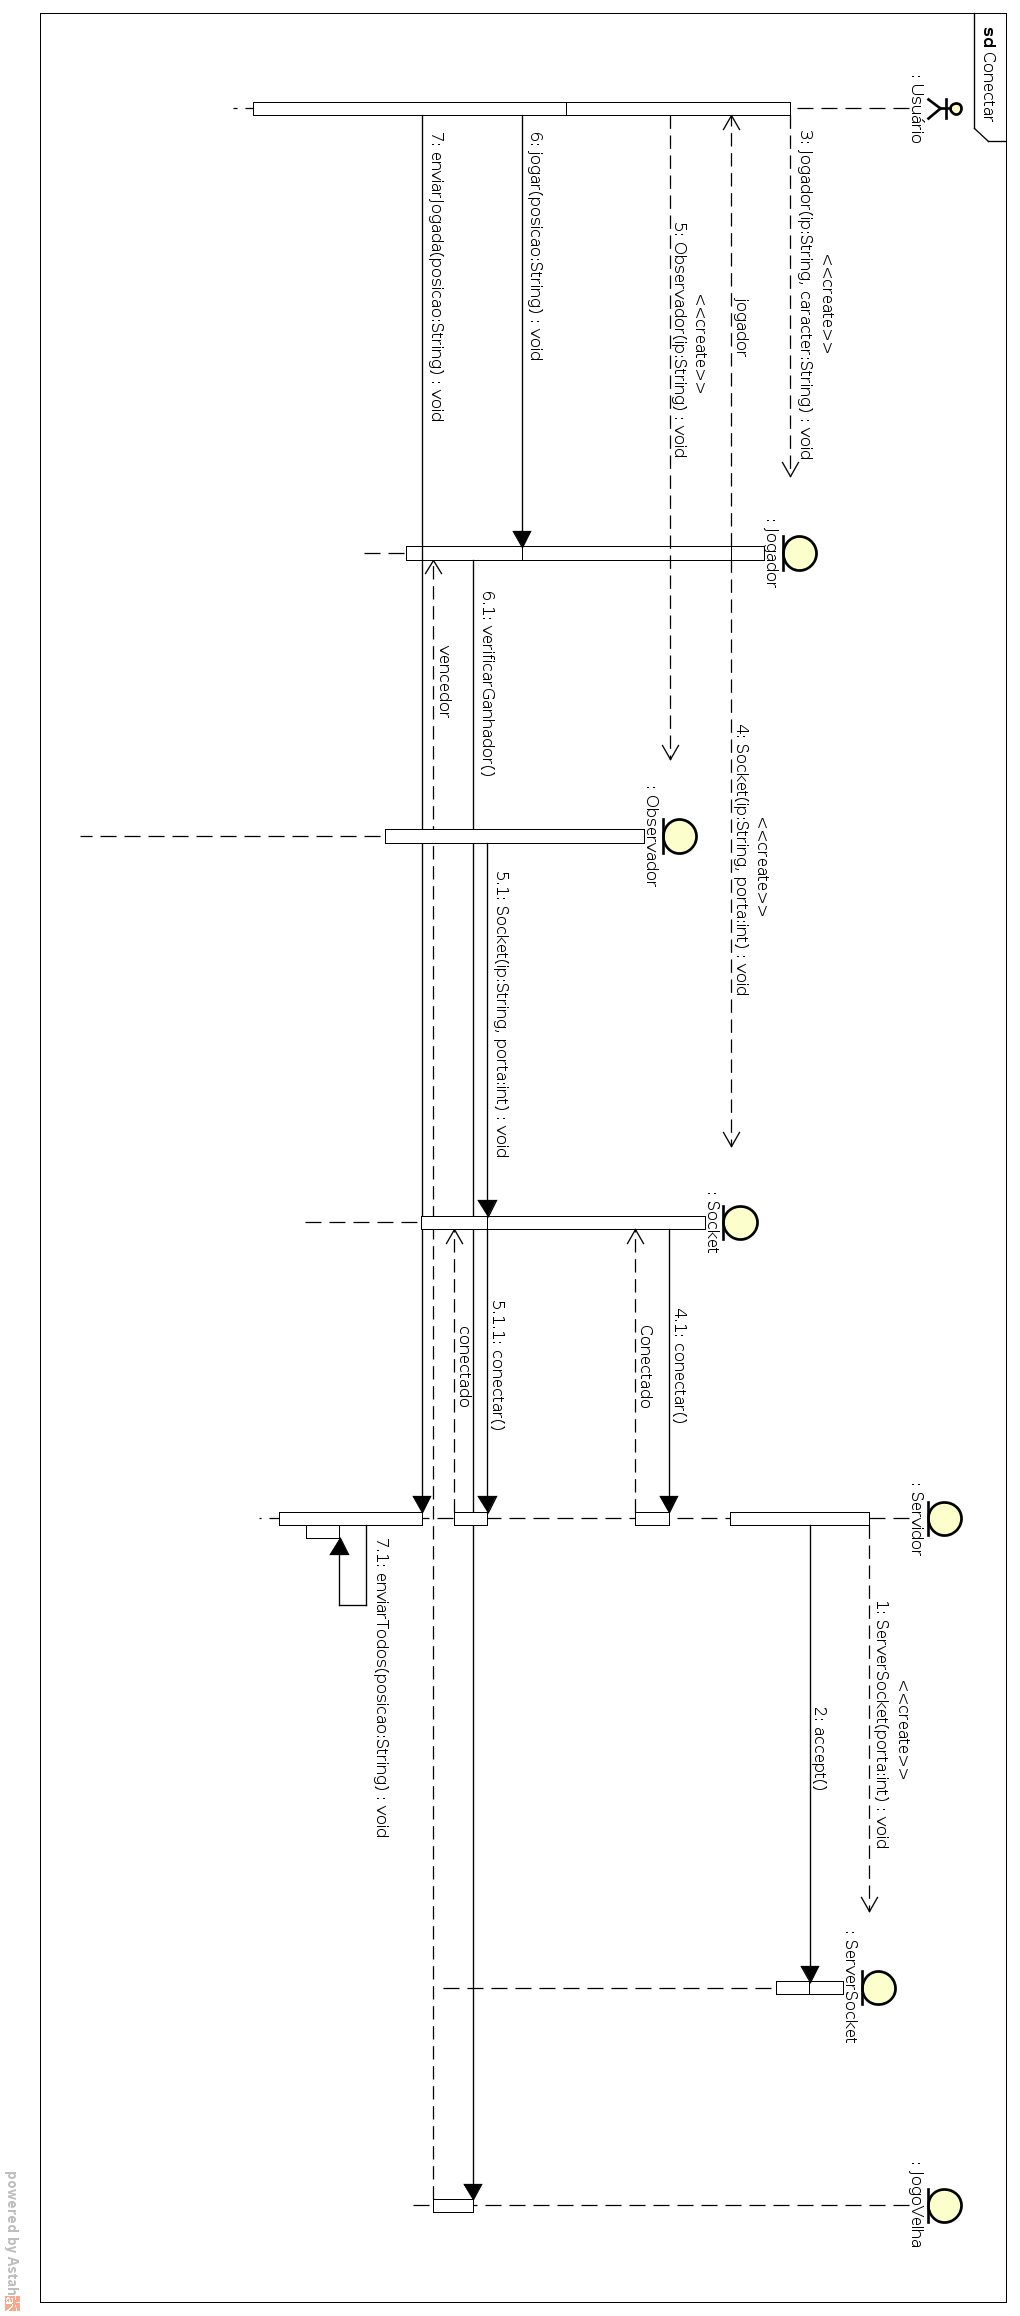
\includegraphics[scale=0.3]{Conectar.png}
	\label{c}
	\caption{Diagrama de Sequência referente à conexão cliente-servidor}
\end{figure}

     
\bibliography{bib}

\end{document}
